\subsection{Definition}
\begin{frame}
  \frametitle{Definition}

  \begin{block}{Zweck}
  	Definition einer 1-zu-n-Abhängigkeit zwischen Objekten, damit im FAll einer Zustandsänderung eines Ojbekts alle davon abhängigen Objekte entsprechend benachrichtigt und automatisch aktualisiert werden.
  \end{block}
  	
  	
  \begin{block}{Motivation}
  	\begin{itemize}
  		\item asdf
  		\item asdf
  	\end{itemize}
  \end{block}
 \end{frame}

\subsection{Klassendiagramm}
\begin{frame}
	\frametitle{Klassendiagramm}
	
	\begin{columns} 
    	\column[c]{.30\textwidth} 
    		\begin{enumerate} 
    			\item privater Konstruktor 
    			\item statische getInstance() Methode zum Zugriff
    		\end{enumerate} 
    	\column[c]{.70\textwidth} 
    			\begin{figure}
					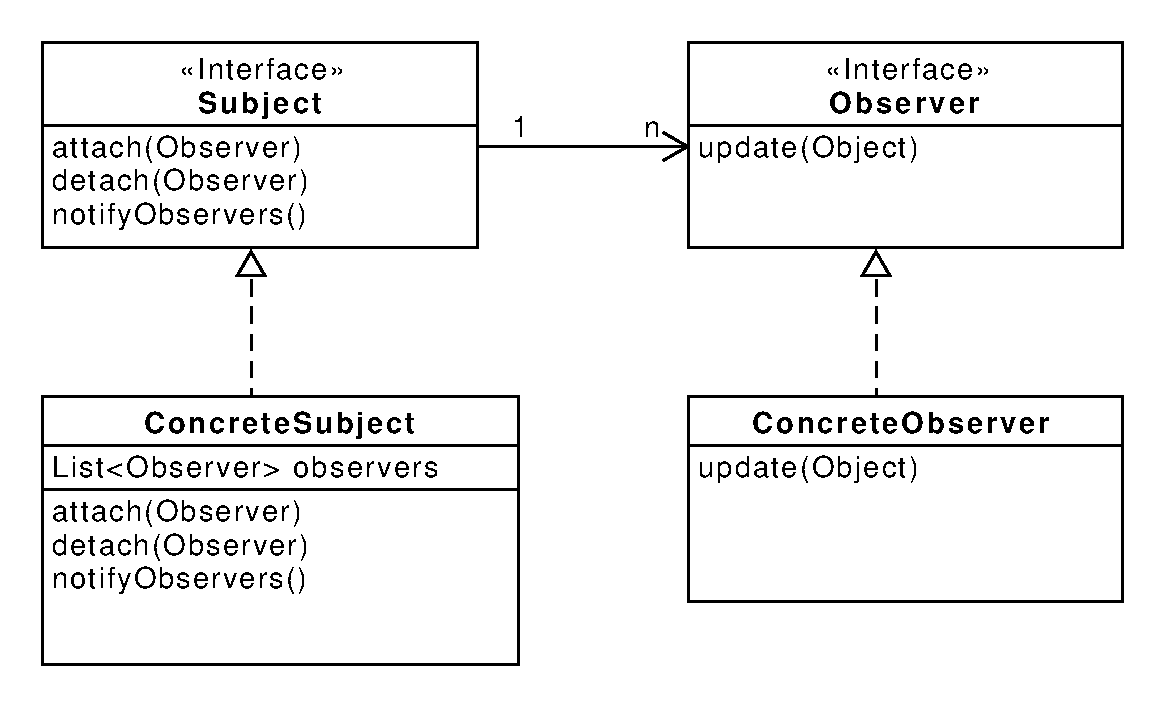
\includegraphics[width=\textwidth]{paper/observer/observer}
				\end{figure}
  	\end{columns} 
\end{frame}

